%===================================== CHAP 5 =================================

\chapter{System Architecture}

\section{Architecture Description}
The project can be divided into back-end and front-end (see fig. \ref{Architecture}).
\\On the back-end, Nginx is used to serve the static files and media requested by the client. All other requests are routed to a server hosted by Django. This server is responsible for routing to sub-pages, authentication and rendering of templates. The SQLite database is also running on this server, providing efficient data flow. The data in the database can only be accessed through the server, making it secure.

On the front-end the client receives files from the server to be displayed in a browser. Some of the files contains components created using the React library. These components take user input, exchange data with the server and display the new information, giving the website a dynamic behaviour.

\begin{figure}[h!]
\centering
    \includegraphics[width=1\textwidth]{fig/Architecture}
\caption{Architecture}
\label{Architecture}
\end{figure}

\section{Back End}
The back end was written in Python (see \ref{python}) with the Django framework (see \ref{django}). The back end is the application's logical layer. The back end communicates with all front end layers, validates information that comes from client and serves the outgoing information to client. Database restrictions are also handled by this layer. All information flow going through the database are created, validated and updated at this stage. 


\subsection{Database Structure}
The database is structured with four different tables; User, UserProfile, Activity and Organisation. These four tables are bounded together by three different relational tables and one single relation between the User table and the UserProfile table. The relational tables are ParticipatedIn, EmployedIn and Hosts (see fig. \ref{Database_Figure}).

The User table is a pre-defined table created by the Django framewor (see \ref{django}). The group chose to use this table to handle User identification. This is a part of Django's security around authentication, and it would require much extra work to write a new secure user authentication system. The client also wanted to divide users into groups, such as a family group. Because of this requirement, the group chose to create a UserProfile table which is dependent on the User table. This allowed for customizing user profiles and creating user groups, without tampering with Django's authentication system. 

The rest of the database works like a normal relational database.

\begin{figure}[h!]
\centering
    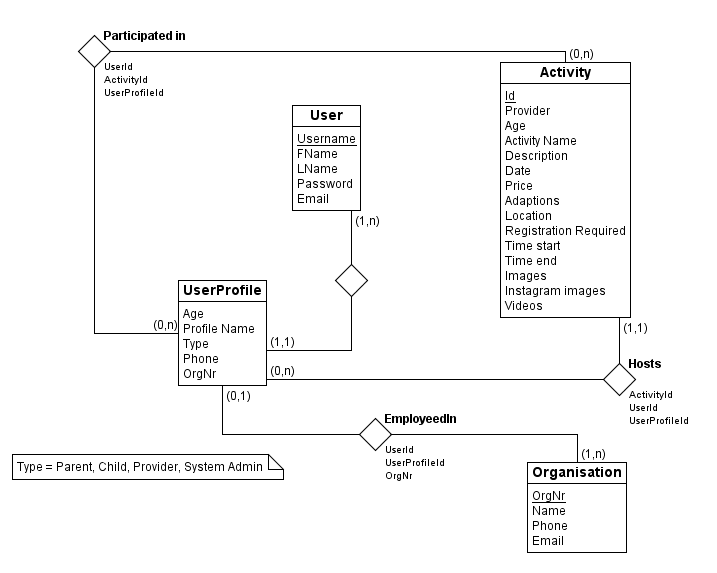
\includegraphics[width=0.85\textwidth]{fig/database_diagram}
\caption{Database structure}
\label{Database_Figure}
\end{figure}


\subsection{Access to Aktørbasen}
A requirement that was made clear, from the beginning of the project and the first meeting with the customer (see \ref{Customer input}), was the need for the web portal to interact with Trondheim Kommune Aktørdatabase. It was important that the leicure activity provoiders that allready was registered in the Aktørdatabbase, could reuse this account or information. such that they don't have to retype allready existing inforamtion. 

Another aspect of the interaction with the Aktørdatabase, is the oppertunity to extract registred leicure activities and leisure clubs. and present them to users through the web portal, and allow users to search for them. Just as a Google search. 

Since the Aktørdatabase is still under development the group had assume, that the Aktørdatabase was to held leisure activities and leisure providers, and after development provide a API that skalvi.no web portal could use, but during development to gain access to the registred information in the Aktørdatabase, the group created a program that queries the official interface for the Aktørdatabase, and then extract the relevant information. This solution is just during development to show the possibility and gain of using the database with skalvi.no. 

During the groups development process the group had a meeting with the developers and project leader of Trondheim Kommune Aktørdatabase, to disguss the oppertunities and later usage of the Aktørdatabase.

\section{Front End}

\subsection{Data Flow}
The data flow figure (see fig. \ref{Data_Flow_Diagram}) was used to help the group members get common understanding of the structure of the web portal. The figure shows where users can navigate within the web portal under different conditions. The figure shows that a user can always navigate to "Front page" and "Activities page", but must be logged in to be able to navigate to "Choose user page" and "My page". Inside "My page" the user can access "Create activity page" and "Edit activity page" if the user is hosting the specific activity. 

\begin{figure}[H]
\centering
    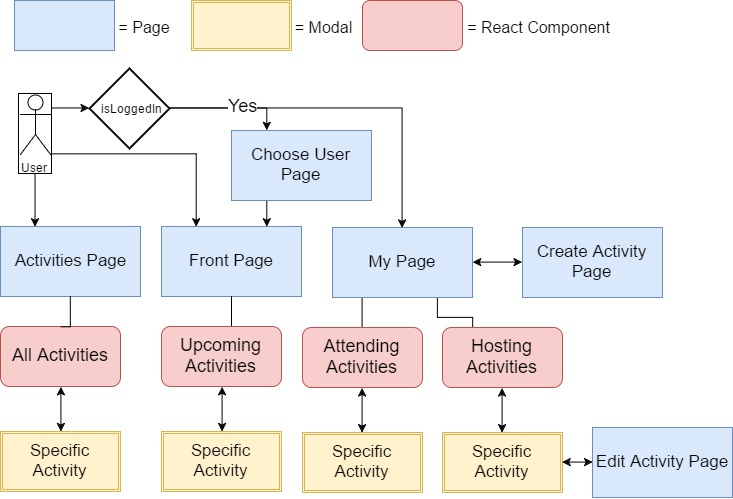
\includegraphics[width=0.9\textwidth]{fig/dataFlow}
\caption{Data Flow}
\label{Data_Flow_Diagram}
\end{figure}

\subsection{Component Diagram}
The web portal contains four different pages (see fig \ref{Component_Diagram}); Front page, Activities page, My page and Create/Edit Activity. Every page contains a navigation bar component for simple navigation, and all pages except Create/Edit Activity have access to different activity components. Only registered users will have access to My page. Each activity component will become a modal if it is clicked, and users that created the activity will be able to edit the activity.

\begin{figure}[H]
\centering
    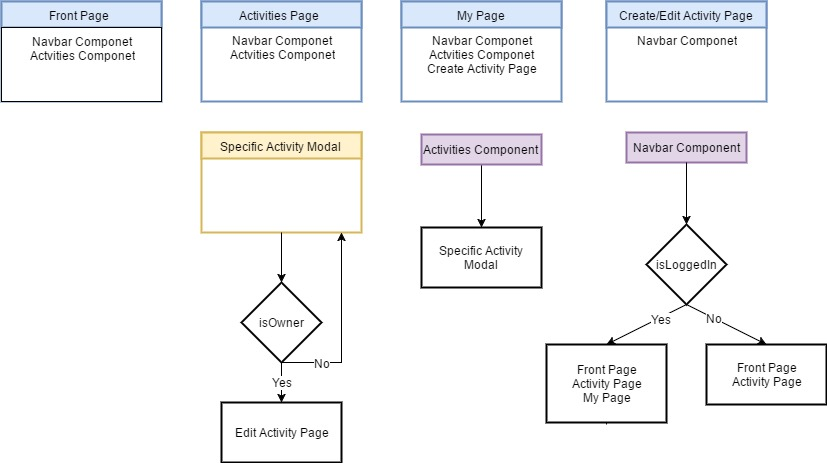
\includegraphics[width=1.0\textwidth]{fig/Component_diagram}
\caption{Component Diagram}
\label{Component_Diagram}
\end{figure}




\subsection{Third Party Interfaces}
In the workshop with the users at the start of the project and during the weekly meetings with the customer, it was often discussed that the web portal should be unique and as easy to use as possible. The users and the customer therefore requested the opportunity to use third party interfaces like Facebook and Instagram in the application. 

\subsubsection{Facebook API}
From the workshop with the users of www.skalvi.no, it was mentioned by several users that they wanted to be able to log in to the web portal with Facebook.
The customer mentioned that many providers use Facebook to display different activities that they offer. He therefore requested the opportunity to create new events in the web portal based on existing Facebook events.  

Based on these requests from the users and the customer, a connection to Facebook's own API was established so that users and providers are able to securely log in to the portal and be able to retrieve events from Facebook. When a user is logged in for the first time, he/she must accept that the web portal can access public profile information and user events.

\subsubsection{Instagram API}
Instagram is a popular society where users can upload and share images and videos. This content is also available by using the API requests defined by Instagram.
An important concept to this project was taking benefit of all the information already available on the web. By connecting the web page to Instagram it allowed the users to use their already existing images when editing or creating an event. 

\subsubsection{Log In}
During the weekly meeting with the customer, he requested that ha wanted a modern way for families to log in. He requested that he wanted families to log in in with one username and password and then be able to select a specific user, similar to the solution that Netflix are using. 

Therefor the opportunity to register user profiles on one specific main user was implemented. When the main user is logging in, it is possible to select which user profile the user wants to use. It is also possible to change user profile at any time.

\section{Graphical User Interface}
The graphical user interface was created in two phases. The first phase was creating a simple paper prototype and the second phase was to develop the user interface with the paper prototype as a template.  

\subsection{Paper Prototype}
During sprint 0 (see \ref{sprint0}) the group designed a paper prototype as the first design of the application. This was a very helpful asset for the group, as it created a common understanding of what was expected to be developed.  

\subsection{User Interface}
The user interface is based on proverbial design principals and uses a lot symbols that users may have encountered earlier on other websites. This is done so users do not have to acquire new knowledge to use the web portal. Universal Design (see \ref{universalDesign}) has also been important during the development of the user interface. This was especially important since the web portals user base was youths with disabilities and disadvantages. 
\cleardoublepage